% !TeX document-id = {05dc9bad-4bec-4210-9b6f-f74d52dfd4d9}
% !TeX TXS-program:compile = txs:///xelatex/[-8bit --shell-escape]
\documentclass{beamer}
\usetheme{AnnArbor}
%\usepackage[spanish]{babel}
%\usepackage{lmodern}
%\usepackage[T1]{fontenc}
%\usepackage[utf8]{inputenc}
\usepackage{fontspec}
\setsansfont{Calibri}
%\setsansfont{Carlito}
%\setsansfont{Raleway}
\setmonofont{Consolas}
\usepackage{xcolor}
\usepackage{amsmath}
\usepackage{amsfonts}
\usepackage{amssymb}
\usepackage{graphicx}
\usepackage{hyperref}
\usepackage{minted}
\usepackage{tikz}
\usepackage{beamerfoils}
\usepackage{hyperref}



\usetikzlibrary{arrows,positioning} 
\tikzset{
	%Define standard arrow tip
	>=stealth',
	%Define style for boxes
	punkt/.style={
		rectangle,
		rounded corners,
		draw=black, very thick,
		text width=6.5em,
		minimum height=2em,
		text centered},
	% Define arrow style
	pil/.style={
		->,
		thick,
		shorten <=2pt,
		shorten >=2pt,}
}




\setbeamerfont{title in head/foot}{size={\fontsize{4pt}{5pt}\selectfont}}
\author{Christian Poveda \& David Cardozo}
% - Give the names in the same order as the appear in the paper.
% - Use the \inst{?} command only if the authors have different
%   affiliation.
\title{An Introduction to Computational Group Theory (GAP) }
\subtitle{Groups, Algorthims, and Programming} % A subtitle is optional and this may be deleted
%\logo{\includegraphics[height=0.8cm]{universidaddelosandes.png}\vspace{220pt}}
\MyLogo{\includegraphics[height=0.8cm]{universidaddelosandesciencias.png}}
\logo{\includegraphics[height=0.8cm]{universidaddelosandesciencias.png}}
%\logo{\includegraphics[height=0.8cm]{universidaddelosandescolombia.png}
\date{\today} % - Either use conference name or its abbreviation.
\subject{PDF Information} % This is only inserted into the PDF information catalog. Can be left out. 
%\setbeamercovered{transparent}
%\setbeamertemplate{navigation symbols}{}

%%Math Stuff

\newtheorem{thm}{Theorem}
\newtheorem{lem}[thm]{Lemma}
\newtheorem{prop}{Proposition}[section]

\theoremstyle{definition}
\newtheorem*{define}{Definition}
\newtheorem{defn}{Definition}[section]
\newtheorem{conj}{Conjecture}[section]
\newtheorem{exm}{Example}[section]
\theoremstyle{remark}
\newtheorem*{rem}{Remark}
\newtheorem{case}{Case}
\newtheorem{exc}{Exercise}
\newtheorem*{sol}{Solution}
\newtheorem*{col}{Corollary}





\begin{document}
\maketitle
\begin{frame}
	\frametitle{What is GAP?}
	\begin{enumerate}[<+->]
		\item \textbf{DIEHTLYAPL}
		\item ``Do I really have to Learn Yet Another Programming Language?''
	\end{enumerate}
	\pause
	\begin{block}{GAP}
		Group, Algorithms, and Programming. Computer algebra system \textbf{CAS}
	\end{block}
	\begin{exampleblock}{Terminal Tool}
		Read input $ \rightarrow $ Evaluate $ \rightarrow  $ Print.
	\end{exampleblock}
	\pause
	\begin{alertblock}{Research Tool}
		You shape it to your needs.
	\end{alertblock}
\end{frame}
\begin{frame}
	\frametitle{Computational Group Theory}
	The study of algorithms for groups. Produce algorithms to answer questions about concrete groups: combinatorial structures.
	\begin{figure}
		\begin{tikzpicture}[node distance=1cm, auto,]
		%nodes
		\node[punkt] (market) {P=NP};
		\node[punkt, inner sep=5pt,below=0.5cm of market]
		(formidler) {Graph Isomorphism [Solved] Travel};
		% We make a dummy figure to make everything look nice.
		\node[above=of market] (dummy) {};
		\node[right=of dummy] (t) {Complexity Theory}
		edge[pil,bend left=45] (market.east) % edges are used to connect two nodes
		edge[pil, bend left=45] (formidler.east); % .east since we want
		% consistent style
		\node[left=of dummy] (g) {Questions Concrete Groups}
		edge[pil, bend right=45] (market.west)
		edge[pil, bend right=45] (formidler.west)
		edge[pil,<->, bend left=45] node[auto] {Can we calculate the objects we define theoretically ?} (t);
		\end{tikzpicture}
	\end{figure}
\end{frame}

\LogoOff
\begin{frame}[fragile]
\frametitle{How to start GAP}
Recall GAP is a command line tool
\begin{minted}[frame=lines, linenos,
numbersep=5pt]{bash}
~$ mkdir ClassTutorial
~$ cd ClassTutorial/
~/ClassTutorial$ gap
┌───────┐   GAP, Version 4.7.5
│  GAP  │   http://www.gap-system.org
└───────┘   Architecture: x86_64...
Libs used:  gmp, readline
Loading the library and packages ...
Components: trans 1.0, prim 2.1, ...
Packages:   Alnuth 3.0.0, AtlasRep 1.5.0 ...
Try '?help' for help. 
gap>
\end{minted}
\end{frame}
\LogoOn
\begin{frame}[fragile]{The GAP console}
Internal types of data structures: Integers are built in, Boolean Values: true, false. And also Gap doesn't need to declare types of variables 
\begin{minted}[frame=lines]{gap}
$ gap>TeachingMode(true);
#I Teaching Mode is turned ON
$ gap>8=9;
false
gap> 1^13 + 12^3 = 9^3 + 10^3;
true
gap> FirstPerfectNumber := 6;
6
gap> 22+FirstPerfectNumber;
28
\end{minted}

\end{frame}
\begin{frame}[fragile]
	\frametitle{Functions}
	GAP comes with a lot of Built-in functions that are commonly used in Group Theory, but it also provide ways to define our own functions.
	\begin{block}{Question}
		Is $ 2^{13} -1 $ a prime number ?
	\end{block}
	\pause
	\begin{minted}{gap}
	gap> IsPrime(2^13 -1);
	true
	\end{minted}
	\pause
	Let us define our own functions:
	\begin{minted}{gap}
	gap> AddOne := function(x) return x+1; end;
	function( x ) ... end
	\end{minted}
	Shortcut: \mintinline{gap}{AddOne:= (x -> x+1);}
\end{frame}
\begin{frame}[fragile]
	\frametitle{Lists}
	Sometimes we will a ``container'' a list structure to keep data. Built-in functions include: Test Membership, and Long List Constructor:
\begin{minted}{gap}
gap> L1 := [4,5,6,7,8,12];
[ 4, 5, 6, 7, 8, 12 ]
gap> Position(L1,7);
gap> List([1..10],x->x);
[ 1, 2, 3, 4, 5, 6, 7, 8, 9, 10 ]
gap> List([5,9..45],x->x);
[ 5, 9, 13, 17, 21, 25, 29, 33, 37, 41, 45 ]
gap> List([20..29],x->x^2);
[ 400, 441, 484, 529, 576, 625, 676, 729, 784, 841 ]
\end{minted}
	Bad Feature on GAP: \textbf{List themselves are pointers to lists}, for copying lists(vector or matrices) \mintinline{gap}{ShallowCopy}
\end{frame}

\begin{frame}[fragile, shrink]
	\frametitle{Vectors and Matrices}
\begin{minted}{gap}
gap> vec := [-1,2,1];
[ -1, 2, 1 ]
gap> M:=[[1,2,3],[4,5,6],[7,8,9]];
[ [ 1, 2, 3 ], [ 4, 5, 6 ], [ 7, 8, 9 ] ]
gap> Display(M);
[ [  1,  2,  3 ],
[  4,  5,  6 ],
[  7,  8,  9 ] ]
gap> vec*M;
[ 14, 16, 18 ]
gap> M*vec;
[ 6, 12, 18 ]
gap> M[3][2];
8
gap> vec*vec; #The inner product
6	
\end{minted}
	While vectors in GAP are usually considered as row vectors, scalar products or matrix/vector products automatically consider the second factor as column vector.
\end{frame}
\begin{frame}
	\frametitle{Hill Cipher}
	Plain text is divided into sets of $ n $ letters, each of which is replaced by a set of $ n $ cipher letters is called a \textbf{polygraphic system}.

\LogoOff

\begin{figure}
\centering
\includegraphics[width=1.3\linewidth]{HillCipher}
\label{fig:HillCipher}
\end{figure}
\begin{thm}
	A \emph{square matrix} $ A $ with entries in $ \mathcal{Z}_m $ is invertible modulo $ m $ if and only if the residue of $ \operatorname{det}(A) $ modulo $ m $ has a reciprocal modulo $ m $
\end{thm}
\begin{col}
	A \emph{square matrix} $ A $ with entires in $ \mathcal{Z}_{26} $ is invertible modulo $ 26 $ if and only if the residue of $ \operatorname{det}(A) $ mod $ 26 $ is not divisible by $ 2 $ or $ 13 $
\end{col}
\end{frame}

\begin{frame}
	\frametitle{Algorithm for the Hill Cipher}
	\begin{enumerate}
		\uncover<1->{\item Choose a $ 2 \times 2 $ matrix with integers:
			\[ A = \begin{pmatrix}
				a_{11} & a_{12} \\
				a_{21} & a_{22}
			\end{pmatrix} \]}
		\uncover<2->{\item Group successive plaintext letter into pairs, adding an arbitrary ``dummy'' letter \textit{mutatis mutandis}, and replace by its numerical value}
		\uncover<3->{\item Successively convert each plaintext pair into a column vector:
			 \[ \vec{p} = \begin{pmatrix}
			 p_1 \\
			 p_2
			 \end{pmatrix} \]
			 Form the product $ A \vec{p} $ the \textbf{ciphertext vector}}
		\uncover<4->{\item Convert each ciphertext vector into its alphabetic equivalent}
	\end{enumerate}
\end{frame}
\begin{frame}[fragile]
	Message to encode: \textbf{I AM HIDING}, using the matrix:
	\[ \begin{pmatrix}
	1 & 2 \\
	0 & 3
	\end{pmatrix} \]
	\begin{table}
		\begin{tabular}{lllll}
			I\,A  & M\,H   & I\,D  & I\,N   & G\,G  \\
			9 \, 1 & 13 \, 8 & 9 \, 4 & 9 \, 14 & 7 \, 7 \\
		\end{tabular}
	\end{table}
	
\begin{minted}{gap}
gap> im:=Integers mod 26; # Represent numbers for mod 26 
gap> A := [[1,2],[0,3]]*One(im);
gap> p1 := [9,1]*One(im);
gap> p2 := [13,8]*One(im);
gap> p3 := [9,4]*One(im);
gap> p4 := [9,14]*One(im);
gap> p5 := [7,7]*One(im);
\end{minted}
\end{frame}
\begin{frame}[fragile,plain]
	\frametitle{Hill Cipher}
\textbf{Hell} 2-\textbf{cipher}
\begin{minted}{gap}
gap> Result := List([A*p1,A*p2,A*p3,A*p4,A*p5],x->x);
gap> Display(Result);
matrix over Integers mod 26:
[ [  11,   3 ],
[   3,  24 ],
[  17,  12 ],
[  11,  16 ],
[  21,  21 ] ]
\end{minted}
\begin{table}
	\begin{tabular}{lllll}
		11\,3  & 3\,24   & 17\,12  & 11\,16   & 21\,21  \\
		K \, C & C \, X & Q \, L & K \, P & U \, U \\
	\end{tabular}
\end{table}
So we will transmit the following:
\centerline{\textbf{KCCXQLKPUU}}
	
\end{frame}

\begin{frame}[fragile]
	\frametitle{Breaking a Hill Cipher}
	
\begin{figure}
\includegraphics[width=0.7\linewidth]{"HillCipherMachine"}
\caption[Hill Machine]{}
\caption{}
\label{fig:HillCipherMachine}
\end{figure}
\end{frame}


\begin{frame}
	\begin{columns}[T] % align columns
		\begin{column}{.48\textwidth}
			\color{red}\rule{\linewidth}{4pt}
			\begin{figure}
				\includegraphics[scale=0.25]{PolishPostcard}
				\caption{Polish Card}
			\end{figure}
		\end{column}%
		\hfill%
		\begin{column}{.48\textwidth}
			Creation of the Republic of Poland, was cumbersome at best. In 1934, a card was intercept from Galicia from a Polish Army officer (some sites mention Edward Rydz-Śmigły ) to Warsaw.
			\color{blue}\rule{\linewidth}{4pt}
			\centering IOSBTHXESPXHOPDE
			
			It was customary in Poland to start a letter with DEAR
		\end{column}%
	\end{columns}
\end{frame}

\LogoOff
\begin{frame}
	\title{Breaking a Hill Cipher}
	It is a basic result in linear algebra that a linear transformation is completely determined by its values at a basis. Thus suggests that if we have a Hill n-cipher, and if $ \vec{p}_1,\ldots \vec{p}_n $ are linearly independent plaintext vectors whose corresponding cipher vectors: $ A\vec{p}_1, \ldots, A \vec{p}_n $ are known, then there is enough information available to determine the matrix $ A $ and hence $ A^{-1} \mod 26 $
	\begin{thm}
		Let $ \vec{p}_1,\ldots \vec{p}_n $ be linearly independent plaintext vectors, and let $ \vec{c}_1,\ldots, \vec{c}_n $ be the corresponding ciphertext vectors in a Hill n-cipher if:
		\[ P = \begin{pmatrix}
		\vec{p}_1^T \\
		\vdots \\
		\vec{p}_n^T
		\end{pmatrix} \quad C =
		\begin{pmatrix}
		\vec{c}_1^T \\
		\vdots \\
		\vec{c}_n^T
		\end{pmatrix} \]
		Where both are $ n \times n $, then the sequence of elementary row operations that reduces $ C $  to $ I $ transforms $ P $ to $ (A^{-1})T $
	\end{thm}
	
\end{frame}

\begin{frame}[fragile]
\begin{minted}{gap}
M := [[9,15],[19,2]]*One(im);
p1:=[4,1]*One(im);
p2:=[5,18]*One(im);
Inverse(M)*p1;
Descipher:=[[1,17],[0,9]]*One(im);
\end{minted}
We end up with the matrix:
\[ A^{-1} = \begin{pmatrix}
1 & 17 \\
0 & 9
\end{pmatrix} \]
\end{frame}


	
\begin{frame}
	\begin{columns}[T] % align columns
		\begin{column}{.48\textwidth}
			\color{red}\rule{\linewidth}{4pt}
			\begin{figure}
				\includegraphics[scale=0.5]{HillBreak}
			\end{figure}
		\end{column}%
		\hfill%
		\begin{column}{.48\textwidth}
			\color{blue}\rule{\linewidth}{4pt}
			Finally we construct the message from the plaintext pairs:
			
			DEAR IKE SEND TANKS.
		\end{column}%
	\end{columns}
\end{frame}

\LogoOn
\begin{frame}[fragile]
	\frametitle{Advanced Group Theory}
	\framesubtitle{Cyclic, Abelian, and Dihedral Groups}
\begin{minted}{gap}
gap> G:= CyclicGroup(6);
<fp group of size 6 on the generators [ a ]>
gap> Elements(G);
[ <identity ...>, a, a^2, a^3, a^4, a^5 ]
gap> List(Elements(G),Order);
[ 1, 6, 3, 2, 3, 6 ]
gap> ShowMultiplicationTable(G);
*    | <id> a    a^2  a^3  a^4  a^5
-----+------------------------------
<id> | <id> a    a^2  a^3  a^4  a^5
a    | a    a^2  a^3  a^4  a^5  <id>
a^2  | a^2  a^3  a^4  a^5  <id> a
a^3  | a^3  a^4  a^5  <id> a    a^2
a^4  | a^4  a^5  <id> a    a^2  a^3
a^5  | a^5  <id> a    a^2  a^3  a^4
\end{minted}
\end{frame}

\begin{frame}[fragile]
	\frametitle{Abelian Group}
	\begin{alertblock}{The Fundamental Theorem Of Finite Abelian Groups}
		A finite Abelian group is isomorphic to a direct product of cyclic groups of prime-power order
	\end{alertblock}
\begin{minted}{gap}
gap> G:=AbelianGroup([2,4,5]);
<fp group of size 40 on the generators [ f1, f2, f3 ]>
gap> gens:= GeneratorsOfGroup(G);
[ f1, f2, f3 ]
gap> List(gens,Order);
[ 2, 4, 5 ]
\end{minted}
\end{frame}

\begin{frame}[fragile]
\frametitle{Working with: $ \left( \frac{\mathbb{Z}}{n\mathbb{Z}} \right)^{\times} $}
\begin{minted}{gap}
gap> G:= Units(Integers mod 21);
<group of size 12 with 2 generators>
gap> e:=Elements(G);
[ ZmodnZObj( 1, 21 ), ZmodnZObj( 2, 21 ), ZmodnZObj( 4, 21 ),
ZmodnZObj( 5, 21 ), ZmodnZObj( 8, 21 ), ZmodnZObj( 10, 21 ),
ZmodnZObj( 11, 21 ), ZmodnZObj( 13, 21 ), ZmodnZObj( 16, 21 ),
ZmodnZObj( 17, 21 ), ZmodnZObj( 19, 21 ), ZmodnZObj( 20, 21 ) ]
gap> List(e,Order);
[ 1, 6, 3, 6, 2, 6, 6, 2, 3, 6, 6, 2 ]
\end{minted}
\pause
\begin{alertblock}{Interpret:}
	\mintinline{gap}{List(e,x->Position(e,Inverse(x)));}
\end{alertblock}

Finally: \mintinline{gap}{gap> ShowGcd(5,9)}

\end{frame}

\begin{frame}[fragile,shrink]
\frametitle{Dihiedral Group and Advanced functions}
This will be short, just to show a few advanced commands:
\begin{minted}{gap}
gap> D3 := DihedralGroup(6);
<fp group of size 6 on the generators [ r, s ]>
gap> D4:=DihedralGroup(8);
<fp group of size 8 on the generators [ r, s ]>
gap> List([D3,D4],x->IsSolvable(x));
[ true, true ]
gap> List([D3,D4],x->IsNilpotent(x));
[ false, true ]
\end{minted}
We can then compute the multiplication table:
\begin{minted}{gap}
gap> ShowMultiplicationTable(DihedralGroup(6));
*    | <id> r^-1 r    s    r*s  s*r
-----+------------------------------
<id> | <id> r^-1 r    s    r*s  s*r
r^-1 | r^-1 r    <id> s*r  s    r*s
r    | r    <id> r^-1 r*s  s*r  s
s    | s    r*s  s*r  <id> r^-1 r
r*s  | r*s  s*r  s    r    <id> r^-1
s*r  | s*r  s    r*s  r^-1 r    <id>
\end{minted}
\end{frame}

\begin{frame}[fragile]
	\frametitle{Subgroups}
	Subgroups in GAP are created and stored by giving generators of the subgroup. The function \mintinline{gap}{Subgroup(group,generators)} constructs a subgroup with given generators. Compared with \mintinline{gap}{Group}, GAP tests whether the generators are actually in the group.
	
	The commands \mintinline{gap}{Normalizer(group,sub)} and \mintinline{gap}{Centralizer(group,sub)} return associated subgroups.
	
	The command \mintinline{gap}{AllSubgroups} should be used with caution:
\begin{minted}[]{gap}
gap> D6:=DihedralGroup(IsPermGroup,6);
Group([ (1,2,3), (2,3) ])
gap> AllSubgroups(D6);
[ Group(()), Group([ (2,3) ]), Group([ (1,2) ]),
 Group([ (1,3) ]), 
 Group([ (1,2,3) ]), 
 Group([ (1,2,3), (2,3) ]) ]
\end{minted}
\end{frame}

\begin{frame}[fragile]
	\frametitle{Subgroup Lattice}
	GAP  provides very general functionality to determine the subgroup structure of a group. To reduce storage this is typically done up to
	conjugacy.
	\mintinline{gap}{ConjugacyClassesSubgroups(G)} returns a list of conjugacy classes of subgroups of $ G $. For each class $ C $ in this list \mintinline{gap}{Representative(C)} returns one subgroup in this class. \mintinline{gap}{Stabilizer(C)} returns the normalizer of this Representative in $ G $. \mintinline{gap}{Size(C)} returns the number of conjugate subgroups
	in the class ( the index of the normalizer). 
	Last but not least, \mintinline{gap}{NormalSubgroups(G)} returns a list of all normal subgroups.
	
\end{frame}

\begin{frame}[fragile]
	\frametitle{Subgroup Lattice II}
\mintinline{gap}{LatticeSubgroups(G)} determines an object L that represents the lattice of subgroups of G .(The classes of subgroups can be also obtained from this object as \mintinline{gap}{ConjugacyClassesSubgroups(L)}.)
For such a lattice object, \mintinline{gap}{MaximalSubgroupsLattice(L)} returns a list $ M $ that describes maximality
inclusion.
\pause
\begin{alertblock}{Activity}
	Let's draw the lattice of $ S_4 $ using GAP
\end{alertblock}
\begin{minted}{gap}
gap> L:=LatticeSubgroups(G);
DotFileLatticeSubgroups(L,"tester.dot");
\end{minted}
This will produce a dot file that can be drawn with:
\begin{minted}{bash}
dot -Teps tester.dot > output.eps
\end{minted}
\end{frame}

\begin{frame}[fragile]
\begin{figure}
	\centering
	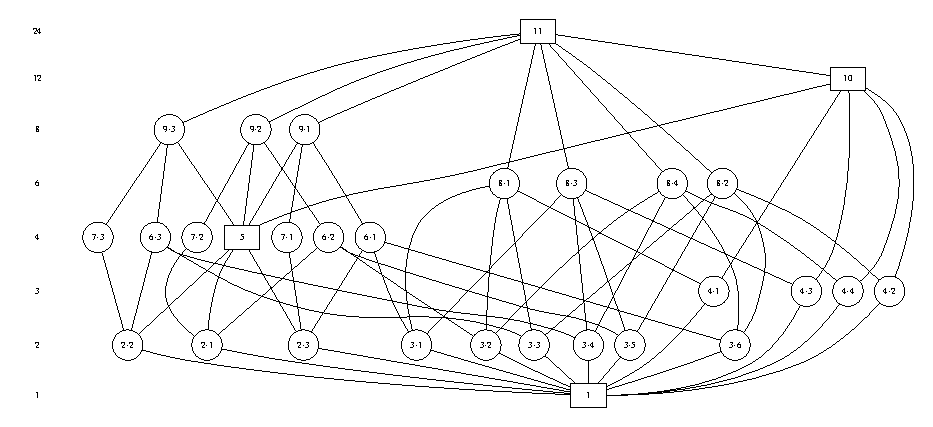
\includegraphics[width=1.0\linewidth]{output}
	\caption{Lattice of $S_4$}
	\label{S4}
\end{figure}

\end{frame}



\begin{frame}
	\frametitle{How we can use GAP to solve puzzles?}
	\framesubtitle{Solving the $ 2 \times 2 \times 2 $ Rubiks cube}
	\begin{columns}[T] % align columns
		\begin{column}{.48\textwidth}
			\color{red}\rule{\linewidth}{4pt}
			\begin{figure}
				\includegraphics[scale=0.4]{Rubik}
			\end{figure}
		\end{column}%
		\hfill%
		\begin{column}{.48\textwidth}
			\color{blue}\rule{\linewidth}{4pt}
			\centering Many puzzles can be described in this way: Each state of the puzzle corresponds to a
			permutation, the task of solving the puzzle then corresponds to expressing the permutation as a
			product of generators.
		\end{column}%
	\end{columns}
\end{frame}

\begin{frame}[fragile]
	\begin{figure}
		\centering
		\includegraphics[scale=0.5]{Rubik}
		\caption{Rubik facelets}
	\end{figure}
\end{frame}


\begin{frame}[fragile]
	We now assume that we will fix the bottom right corner (i.e. the corner labelled with $16/19/24$) in
	space – this is to make up for rotations of the whole cube in space. We therefore need to consider
	only three rotations, front, top and left. The coresponding permutations are (for clockwise rotation
	when looking at the face):
\begin{minted}{gap}
gap> top:=(1,2,4,3)(5,17,13,9)(6,18,14,10);;
gap> left:=(1,9,21,20)(5,6,8,7)(3,11,23,18);;
gap> front:=(3,13,22,8)(4,15,21,6)(9,10,12,11);;
gap> cube:=Group(top,left,front);
Group([(1,2,4,3)(5,17,13,9)(6,18,14,10),(1,9,21,20)(3,11,23,18)(5,6,8,7),
(3,13,22,8)(4,15,21,6)(9,10,12,11) ])
gap> Order(cube);
3674160
\end{minted}
\end{frame}

\begin{frame}[fragile]
	By defining a suitable mapping first (for the time being consider this command as a black box) we
	can choose nicer names – T, L and F – for the generators:
\begin{minted}{gap}
gap> map:=EpimorphismFromFreeGroup(cube:names:=["T","L","F"]);
[ T, L, F ] -> [ (1,2,4,3)(5,17,13,9)(6,18,14,10),
(1,9,21,20)(3,11,23,18)(5,6,8,7), (3,13,22,8)(4,15,21,6)(9,10,12,11) ]
\end{minted}
	We now can use the command Factorization to express permutations in the group as word in
	generators. The reverse sequence of the inverse operations therefore will turn the cube back to its
	original shape.
\end{frame}
\LogoOff
\begin{frame}[fragile]
	\frametitle{How we can use GAP to solve puzzles?}
	\framesubtitle{Solving the $ 2 \times 2 \times 2 $ Rubiks cube}
	\begin{columns}[T] % align columns
		\begin{column}{.48\textwidth}
			\color{red}\rule{\linewidth}{4pt}
			\begin{figure}
				\includegraphics[scale=0.4]{Rubik2}
			\end{figure}
		\end{column}%
		\hfill%
		\begin{column}{.48\textwidth}
			\color{blue}\rule{\linewidth}{4pt}
			\centering This corresponds to the permutation.
			\begin{minted}{gap}
gap> move:=(1,15,20,4,6,2,21)
(3,17,8,5,22,7,13)
(9,14,11,18,12,23,10)
			\end{minted}
			 We express
			 this permutation as word in the generators:
			 \begin{minted}{gap}
gap> Factorization(cube,move);
T*F*L*T*F*T
			 \end{minted}
			 We can thus bring the cube back to its original position by turning each counterclockwise top,front,top,left,front,top.
		\end{column}%
	\end{columns}
\end{frame}


\end{document}	